\section{Iteration 7: Decomposition of the Outbound Communication Scheduler}
\label{add:it7}

\subsection{Step 1: Identify candidate drivers}
\label{add:it7/drivers}

\npar It is crucial that ``shut down valve" trames are sent in time to the
correct module considering that trames that arrive too late can ultimately
lead to a potential disaster claiming the lifes of several people. Therefore the
outbound trames (i.e. towards modules) need to be scheduled. 

\npar The (only) driver of this iteration is 

\begin{itemize}
  	\item P1': Timely closure of valves.
  	\begin{itemize}
  		\item Alarm trames have to be handled within a bounded time. 
    \end{itemize}
\end{itemize}

\npar No use cases were delegated to this scheduler.

\subsection{Step 2: Choose design concepts}
\label{add:it7/concepts}

\npar The design concepts for this decomposition are exactly the same as those
of the storage and anomaly detection scheduler, see sections
\ref{add:it3/concepts} and \ref{add:it5/concepts}.
This is a logical result considering that both schedulers are established with
performance drivers in mind.

\subsection{Step 3: Instantiate architectural elements and allocate responsibilities}
\label{add:it7/elements}

\begin{figure}[H]
	\begin{centering}
		% TODO Figure
		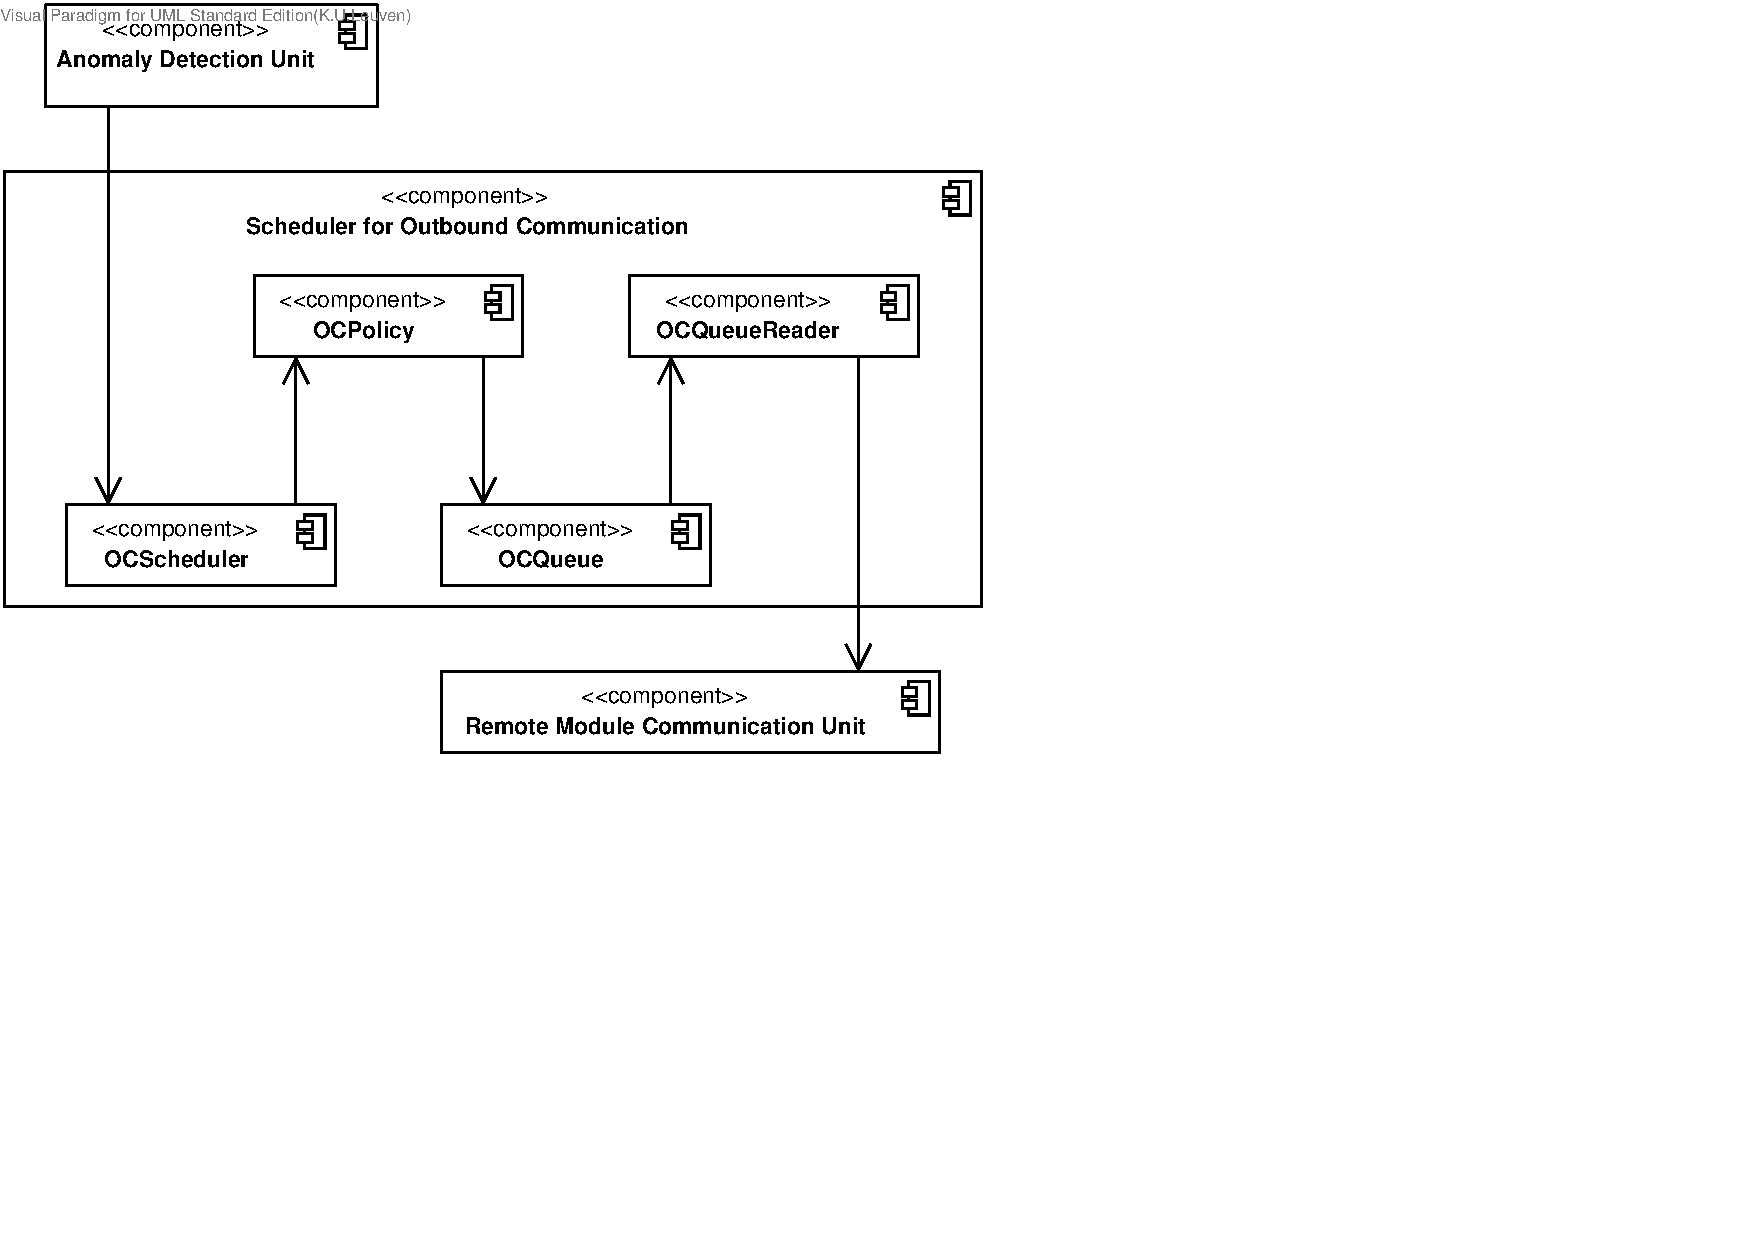
\includegraphics[width=\textwidth]{figs/add-it7-elements.pdf}
		\caption{Overview of the instantiated child elements in the Outbound
		Communication Scheduler}
		\label{fig:it7/elements}
	\end{centering}
\end{figure}

\npar The design of the outbound communication scheduler is analogous to that
of the storage scheduler and the anomaly detection scheduler. This is rather
locical because they all have the same purpose: schedule commands of some kind.

\npar All requests to the Outbound Communication Scheduler are encapsulated as
OCCommand objects. These objects represent requests to send a certain control
trame to a given remote device for some reason. 

\npar The scheduler (OCScheduler) handles every incoming command
(OCCommand) by inserting the command in a queue (OCQueue) with a
certain priority using a policy (OCPolicy). The scheduling policy
determines the priority of the command based on the nature of that command
(in particular, the reason for the request). As before, priorities of commands
already in the queue are increased every time a new command is inserted.
Again, this is done to prevent starvation.

\npar An additional component (OCQueueReader) will pop the command with the
highest priority off the queue and present it on the database for execution.

\subsection{Step 4: Define interfaces for instantiated elements}
\label{add:it7/interfaces}

\subsubsection{OutboundCommScheduler}

\paragraph{OutboundTrameScheduler}

\npar The OutboundTrameScheduler was already discussed in section
\ref{add:it1/interfaces}.

\subsubsection{Scheduler}

\npar This component offers no interface.

\subsubsection{PriorityQueue}

\paragraph{OutboundQueue}

\npar This interface is analogous to the priorityqueue interface of the storage
scheduler, see section \ref{add:it3/interfaces}. It offers a \method{pop(trame)}
and \method{push{trame}} method which will respectively pop and push a given
trame from the priorityqueue.

\begin{figure}[H]
	\begin{centering}
		% TODO Figure
		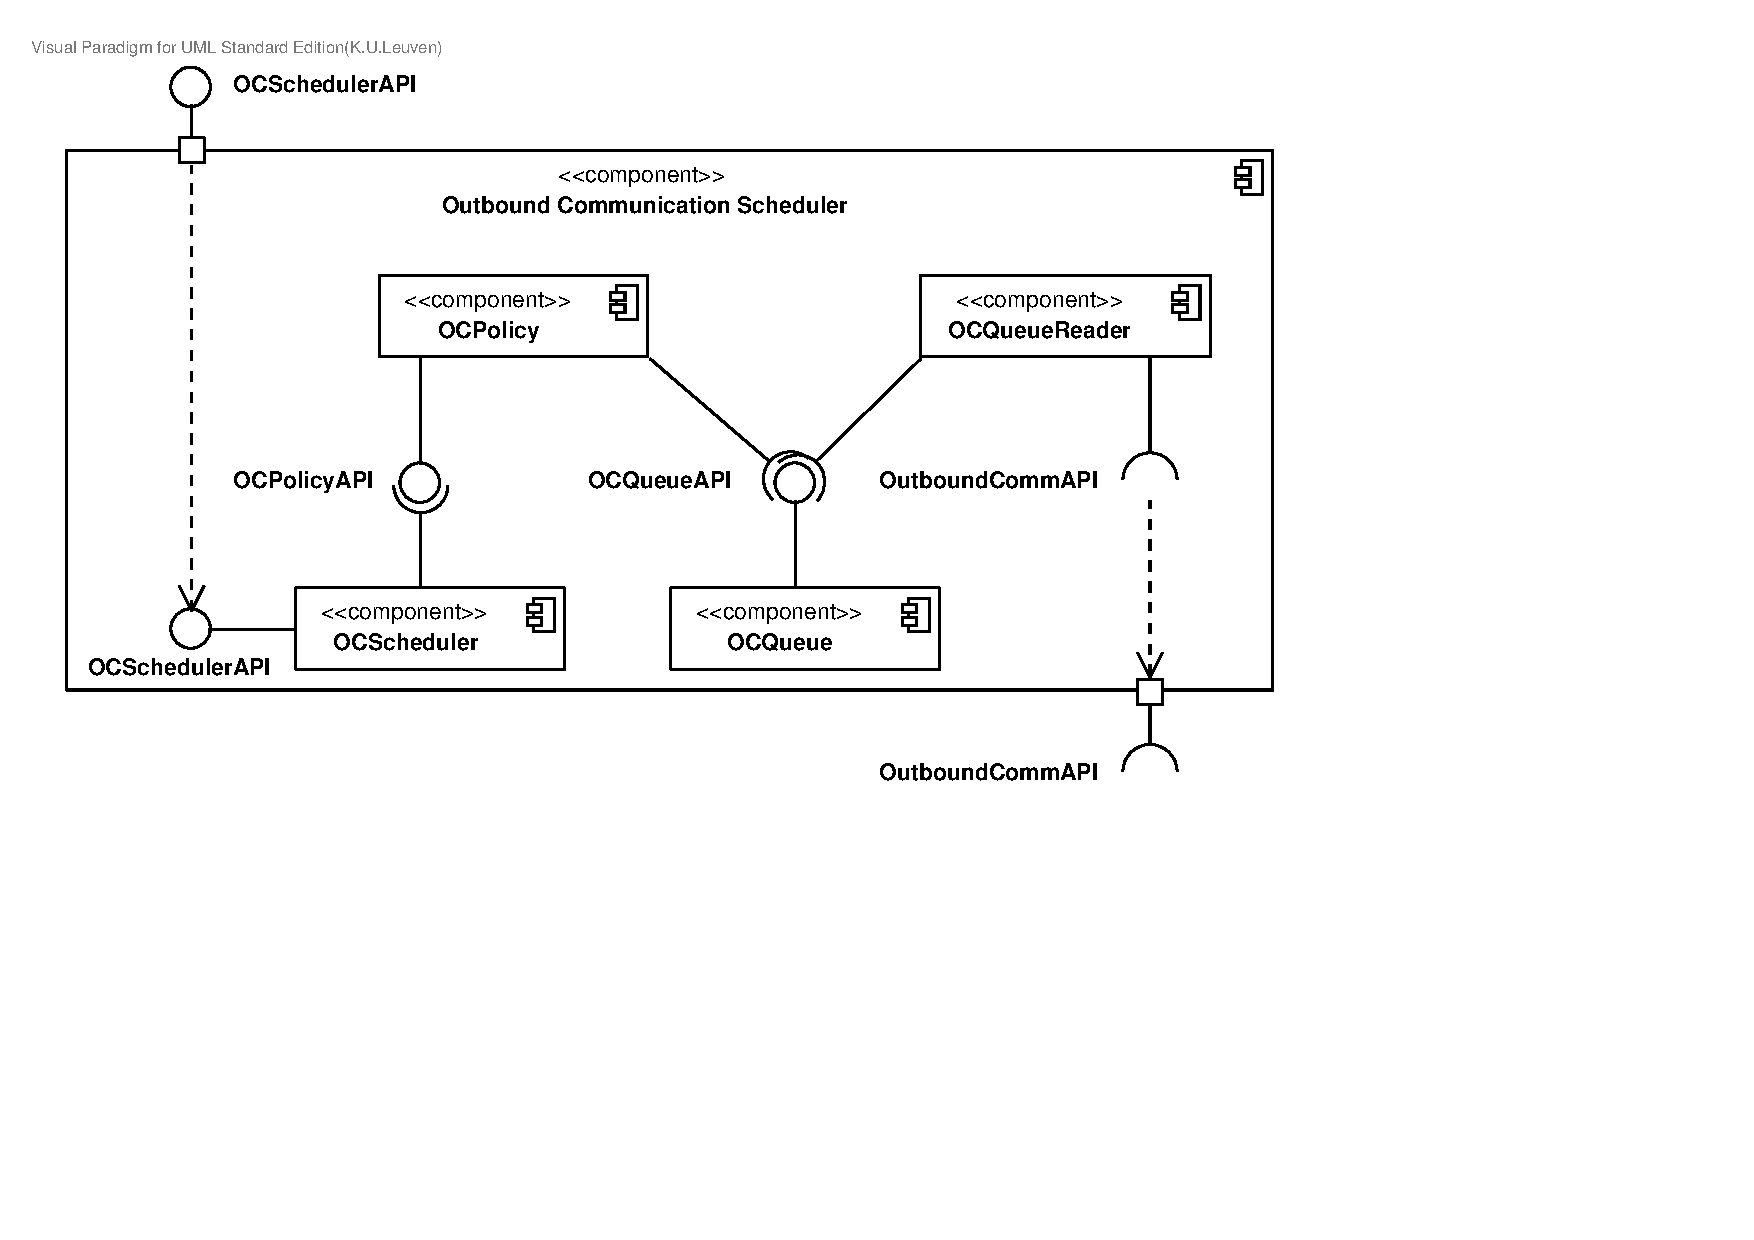
\includegraphics[width=\textwidth]{figs/add-it7-interfaces.pdf}
		\caption{Overview of the interfaces and components in the
		Outbound Communication Scheduler}
		\label{fig:it7/interfaces}
	\end{centering}
\end{figure}

\subsection{Step 5: Verify and refine}
\label{add:it7/verification}

\npar The driver for this iteration, P1, is resolved. The scheduler policy will
prioritize outbound messages that are intended to close valves after an anomaly
is detected.
